\newpage
%%%%%%%%%%%%%%%%%%%%%%%%%%%%%%%%%%%%%%%%%%%%%%%%%%%%%%%%%%%%%%%%%%%%%%%%%%%%%%%
\section{Week 10}
%%%%%%%%%%%%%%%%%%%%%%%%%%%%%%%%%%%%%%%%%%%%%%%%%%%%%%%%%%%%%%%%%%%%%%%%%%%%%%%
\subsection*{Monday, 05/13/2024}
\begin{itemize}
    \item cleaned up the repo a bit and am testing the diesel orm for articles.
    \item lessgo Figure~\ref{fig:diesel_dummy_article}. Oops, 
        \texttt{is_default} should be t for me, will fix.
        \begin{figure}[ht]
            \centering
            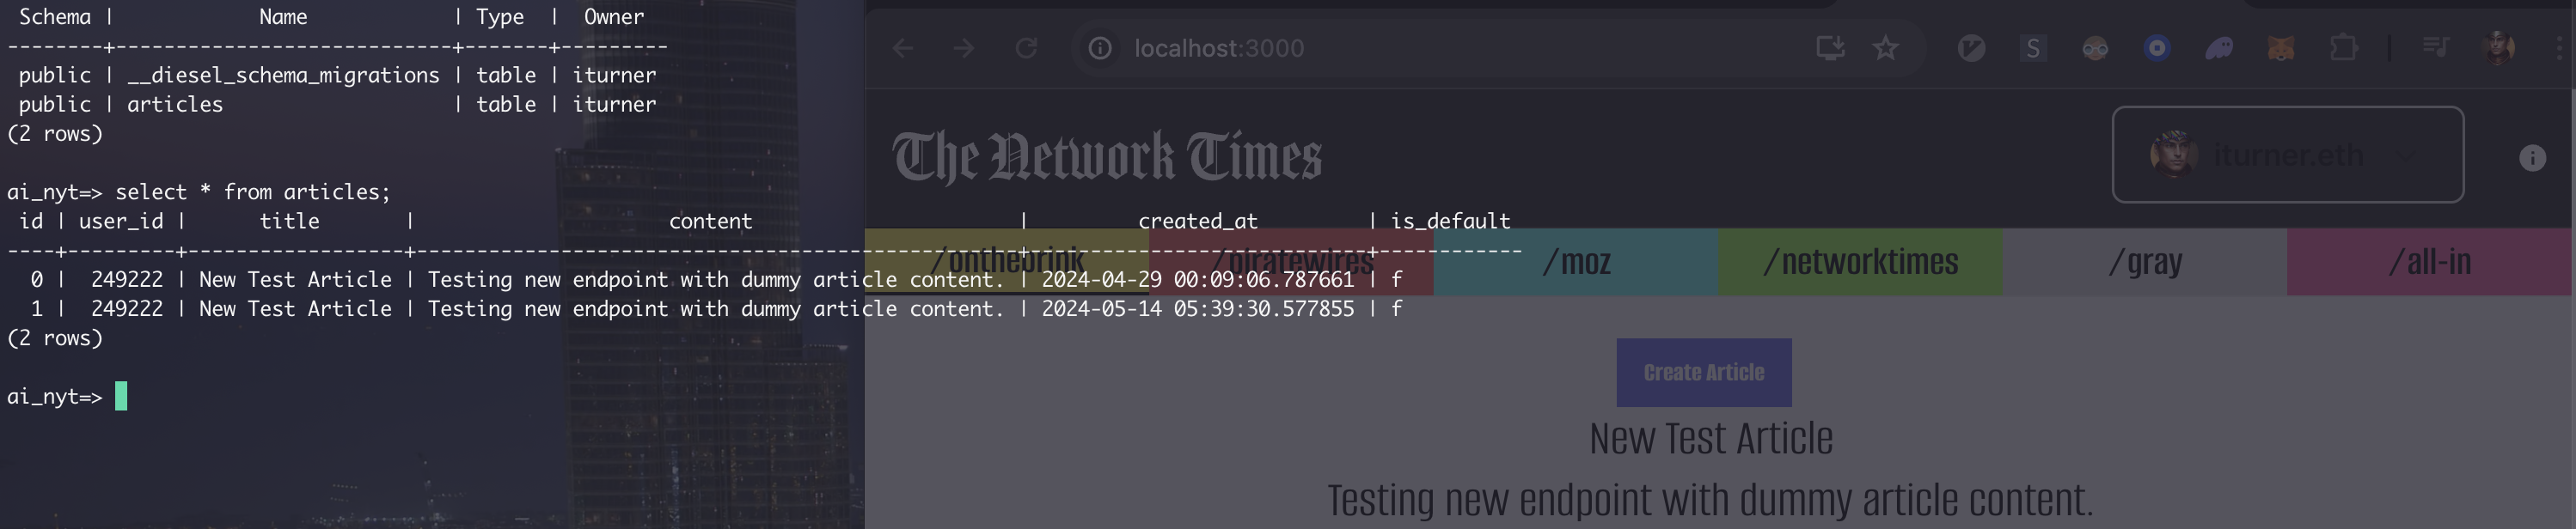
\includegraphics[width=15cm]{diesel_dummy_article}
            \captionsetup{labelfont=bf, textfont=it}
            \caption{Diesel Dummy Article Test}
            \label{fig:diesel_dummy_article}
        \end{figure}
    \item fixed: Figure~\ref{fig:diesel_is_default}.
        \begin{figure}[ht]
            \centering
            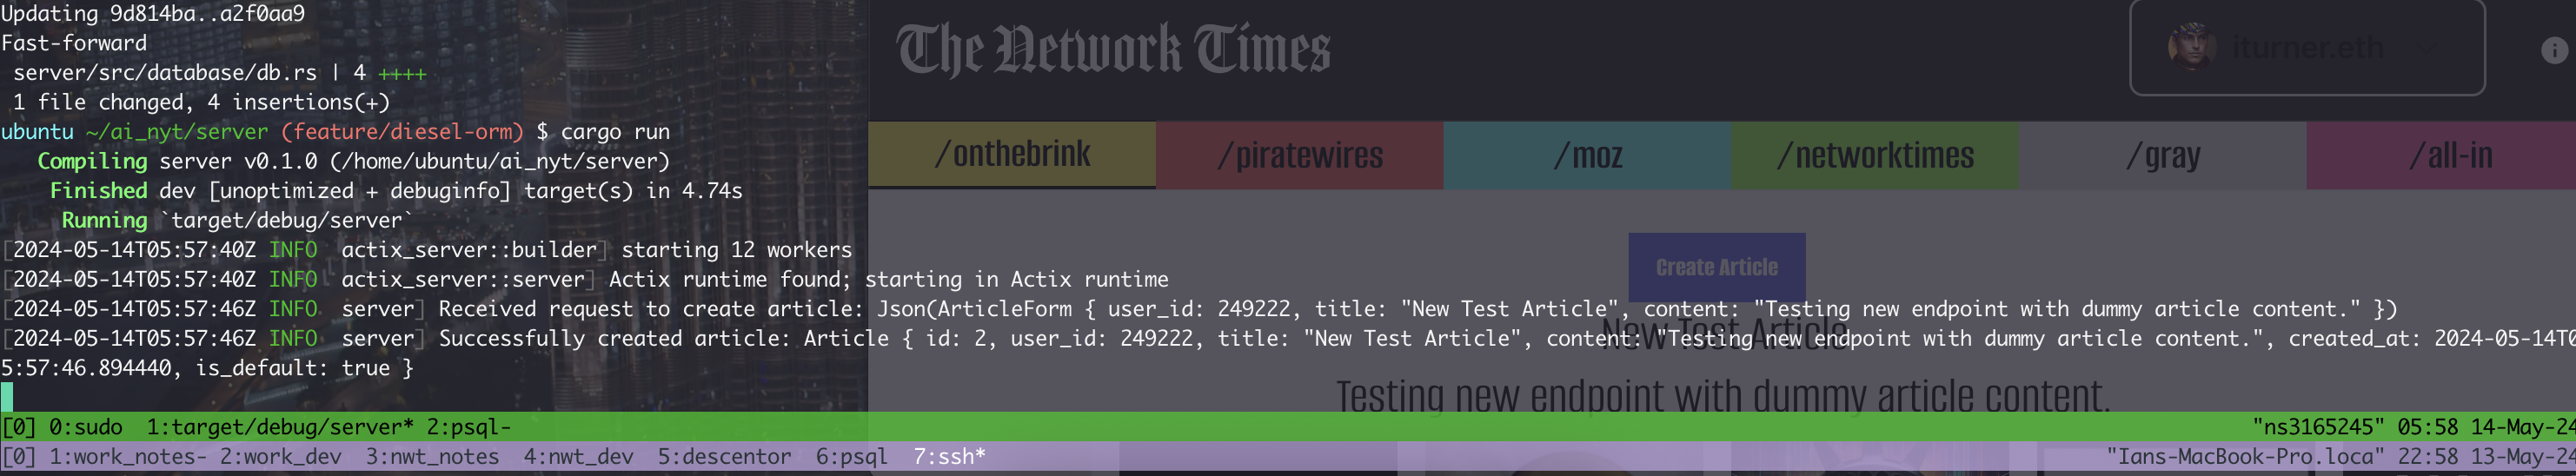
\includegraphics[width=15cm]{diesel_is_default}
            \captionsetup{labelfont=bf, textfont=it}
            \caption{Article \texttt{is_default} Field Working}
            \label{fig:diesel_is_default}
        \end{figure}
    \item spent far too much time prop drilling when it really isn't needed for
        this feature... sigh. I'll just allow the user to save the article or
        not on the Article Page itself.
\end{itemize}
